\chapter{Individual Cetacean ID via Automatic Most Likely Catalogue Matching}\label{ch:ID}

This chapter examines the final component in the automatic photo-id pipeline, focussing on individual identification. The component takes as input photo-id catalogue images which have been passed through the dorsal fin detector and post-processing methodology outlined in Chapter \ref{ch:cetDet} to produce a list of most likely catalogue matches. It is important to note here that this component is not intended to replace photo-id researchers by performing the job for them. Instead, the component aims to vastly reduce the search space the researcher needs to examine in order to verify a catalogue match; a list of most likely matches is suggested, but ultimately the final decision lies with the researcher.

To begin, the requirements an automatic most likely catalogue matching system must meet are outlined. The chapter then discusses possible approaches to the problem and justification for the selected approach. Model development is discussed in detail, using the NDD AU SMRU dataset created in Section \ref{ch:postProcessing,sec:NDD_AU_SMRU} for training and evaluation. The effect of class structure and how this impacts most likely catalogue matching accuracy is discussed, alongside the current limitations of the approach. 

\section{Most Likely Catalogue Matching System Requirements}\label{ch:ID,sec:Requirements}

Before development can begin, it is important to outline the system requirements. Unlike the detector which could be considered a coarse-grained task, identification of individual cetaceans is an extreme fine-grained problem as they are distinguished from each other using small prominent markings present on the dorsal fin. As the animals are free roaming, there can be high variation in how the fin is captured in the image, discussed in greater detail in Section \ref{ch:cetDet,sec:requirements,sub:environmental}. This can lead to photo-id catalogues with low inter-class but high intra-class differences between the individuals present, seen in Figure \ref{fig:segmented-ndd20-example}. As a result of this, any system capable of accurate catalogue matching must be able to recognise these minute differences between individuals even when there is high variation in the examples for each individual class. 

The system must also be capable of operating using all information provided to it. Other photo-id aids which perform most likely catalogue matching such as finFindR \cite{thompson_finfindr_2022} operate using only the trailing edge of the fin, with matching performed using notches and shape. This misses other prominent markings such as long term scarring or pigmentation, as well as the shape of other fin edges. As such, it may be the case that finFindR struggles when operating over a catalogue with few to no notches. To avoid this issue, the system developed must be capable of matching using all available prominent markings. 

Further, the system must also be capable of performing accurate catalogue matching under the presence of noise, both classified and misclassified. Datasets developed for the training of this system such as NDD AU SMRU contain a \texttt{noise} class which encapsulates all detected mask components which are erroneously retained after post-processing has been applied. This class has extremely high intra-class variance, however it is imperative the system is able to match erroneous components to it. Misclassified noise is defined as that which has been passed downstream as a result of being attached to a valid individual detection mask. In Figure \ref{fig:crop-with-unclassified-noise} for example, the swell captured in the post-processed crop would be considered misclassified noise. Any system performing automatic most likely catalogue matching must be resistant to small amounts of misclassified noise in order to produce accurate identity suggestions.

\begin{figure}
	\begin{center}
		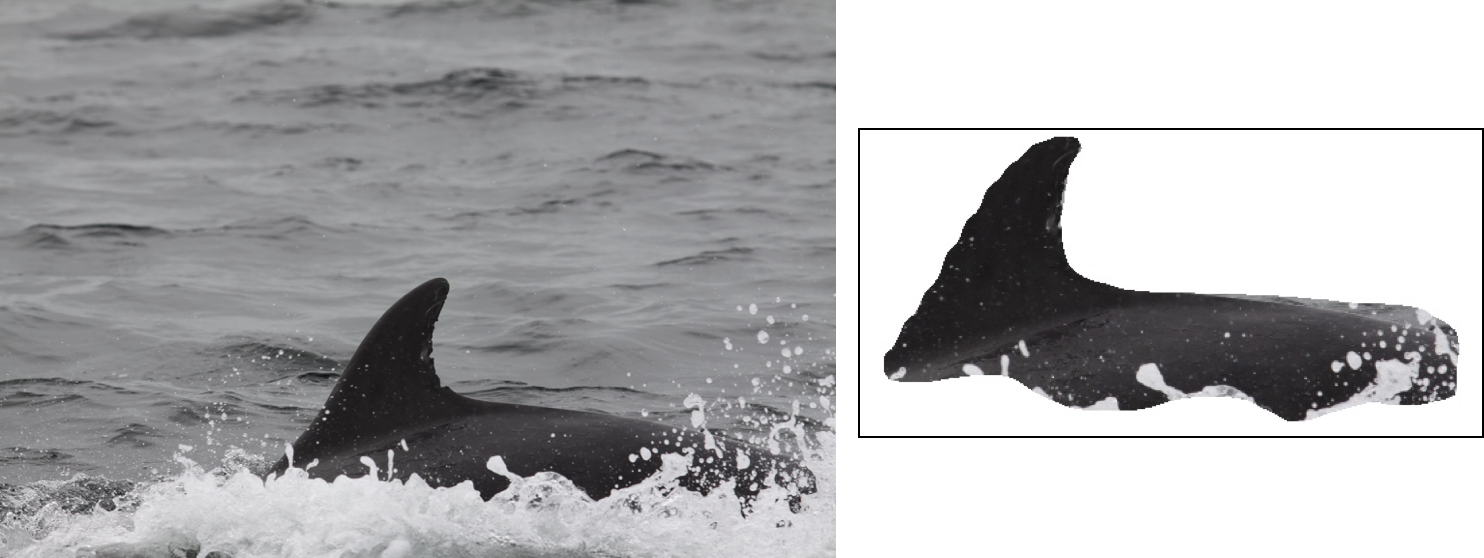
\includegraphics[scale=0.6]{Chapter6/figs/crop-with-unclassified-noise-updated.png}
	\end{center}
	\caption{Left: An example input image. Right: The corresponding post-processed crop which contains some misclassified noise.}
	\label{fig:crop-with-unclassified-noise}
\end{figure}

Any developed system must also be capable of handling examples of individuals which are not present in the photo-id catalogue. Due to the free roaming nature of cetaceans (or indeed any wild animal) and the limitations on photo-id survey size dictated by both weather and workforce, there is no guarantee that every animal who makes use of the survey area will be captured. New animals may also become resident in the area through birth or migration. When these animals are eventually captured during a survey and their image processed, the system must be capable of recognising this as an individual not currently present in the catalogue and highlight this to the researcher. This is made more difficult given the extreme fine-grained nature of the catalogues. As a result, this requirement necessitates that the system must be capable of recognising uncertainty or understand a notion of similarity between an input and the class examples present in the catalogue. 

Traditional computer vision classification models do not meet this requirement. If an example image of a new individual was seen by a traditional CNN trained on a photo-id catalogue dataset, this model would still attempt to provide a classification based on the classes present at train time.  As deep learning based vision models operate on point estimations of parameters, unlike Gaussian processes where the probability distribution is defined over a function, this removes the ability to produce helpful indicators of uncertainty such as prediction confidence bounds \cite{gal_uncertainty_2016}. 

\section{Siamese Neural Networks}\label{ch:ID,sec:deciding,sub:SNN}

Rather than producing a direct classification, Siamese Neural Networks (SNNs) aim to incorporate the notion of similarity into the model. This is achieved by connecting two or more identical CNNs in parallel, each sharing the same backbone architecture, initial and updated weights, and hyperparameters. Each CNN in the SNN is designed to produce an embedding, or a $d$-dimensional representation, of the input. The size of this embedding is set via hyperparameter and dictates how many $d$ dimensions the output of the SNN will be. For example, if an SNN is created with an embedding size of 10, each CNN may take a high dimensional input of size \textit{width} * \textit{height} * \textit{channels} and output a 10-dimensional embedding, a float vector of size 10 which represents the input image. A visualisation of a two branch SNN can be seen in Figure \ref{fig:signet-SNN-architecture}.

\begin{figure}
	\begin{center}
		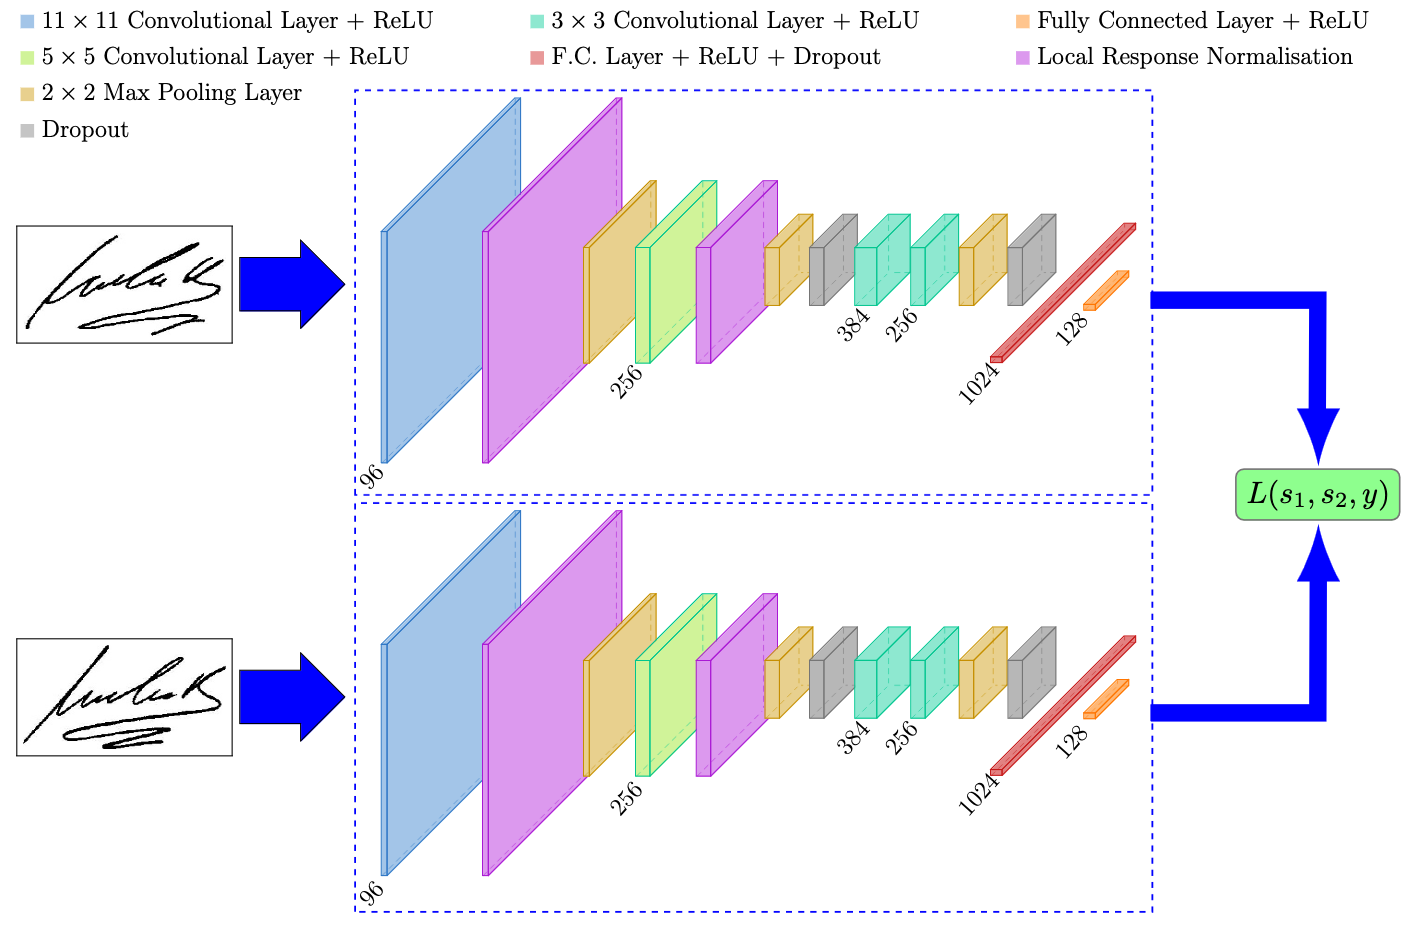
\includegraphics[width=0.8\linewidth]{Chapter6/figs/signet-SNN-architecture.png}
	\end{center}
	\caption[An example two-branch SNN architecture for signature verification.]{An example two-branch SNN architecture for signature verification. Each branch takes as input an image of a signature and passes this through a CNN, where each branch's CNN is identical. A 128-dimensional embedding is produced as output by each branch. Embeddings are then compared using some loss function, $L$, to generate a similarity value. Image from \cite{dey_signet_2017}.}
	\label{fig:signet-SNN-architecture}
\end{figure}

At train time, each CNN branch receives a different image and generates an embedding. These embeddings are compared to one another in order to optimise a loss function, whereby input images of the same class have similar embeddings but those of different classes are dissimilar. In this way the SNN can be tuned to provide a measure of image similarity. Once trained only one branch of the model is retained, allowing a single image to be embedded by the model into the same embedding space and compared to previously embedded images.

It is this ability that has resulted in the widespread use of SNNs for verification or identification problems in computer vision \cite{dey_signet_2017, wang_discriminative_2020}. Specifically in ecology, SNNs have found use in fine-grained species identification problems \cite{vetrova_hidden_2018, araujo_two-view_2022} as well as in more extreme fine-grained individual animal identification \cite{clapham_automated_2020} and behaviour classification \cite{brookes_triple-stream_2023}. 

\subsection{Clustering Embeddings in a Latent Space}\label{ch:ID,sec:deciding,sub:SNN,subsub:ClusteringEmbeddings}

By storing the embeddings generated for each trained class it is possible to produce a list of likely class predictions for a new image by measuring the distance between the generated embedding and those previously produced when plotted into some $d$-dimensional latent space. This thesis makes use of Euclidean distance measurement, though the use of cosine distance measurement is also present in the literature \cite{maharani_improving_2020, pan_towards_2020, feng_triplet_2020}. If the SNN has trained in such a way as to produce low intra-class, high inter-class difference between generated embeddings then this will create class clusters when plotted in the latent space. 

An example of this behaviour can be seen in Figure \ref{fig:mnist-class-clusters-PCA} which shows a 2-dimensional visualisation, produced using Principal Component Analysis (PCA), of the embedding locations for a subset of the MNIST dataset \cite{lecun_gradient-based_1998}. Here, an SNN has been trained for 100 epochs using a Triplet Ranking Loss (outlined in Section \ref{ch:ID,sec:SNNBackground,sub:lossFunction,subsub:Triplet}) to generate embeddings of images for the 10 unique classes. As can be seen, the model is able to generate embeddings in such as way as to cluster those of the same class in the latent space. Note that some clusters are visualised on top of each other due to the dimensionality reduction performed in order to show the latent space on the page. 

\begin{figure}
	\begin{center}
		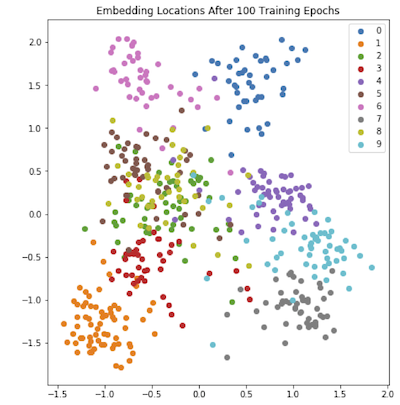
\includegraphics[scale=0.5]{Chapter6/figs/mnist-class-clusters-PCA.png}
	\end{center}
	\caption[A 2-dimensional visualisation of a multi-dimensional latent space produced by an SNN trained on the MNIST dataset for 100 epochs.]{A 2-dimensional visualisation of a multi-dimensional latent space produced by an SNN trained on the MNIST dataset \cite{lecun_gradient-based_1998} for 100 epochs.}
	\label{fig:mnist-class-clusters-PCA}
\end{figure}

It is important to note here that the value of the embeddings is not necessarily important, just the distances between them. Notice how all points in Figure \ref{fig:mnist-class-clusters-PCA} lie within approximately -1.5, 2.0 on the x-axis and -2.0, 2.0 on the y-axis. There is nothing inherently good or bad about an SNN that embeds within this range, all that matters is the points are clustering in their respective classes.

\subsection{Meeting the Outlined Requirements}\label{ch:ID,sec:deciding,sub:SNN,subsub:meetingOutlinedRequirements}

The computational expense of performing inference with an SNN is relatively small. Whilst training requires the use of a branched CNN architecture in order to optimise the loss function, this is reduced to just one branch at inference time. Generating a list of most likely catalogue matches would only require an image to be passed through the network once in order to generate an embedding, and similarity via Euclidean distance measurement in the latent space is cheap to perform. As such, producing a list of most likely catalogue matches is overall computationally efficient using SNNs. 

The clustering of class embeddings in the latent space also allows for easy identification of potential previously uncatalogued individuals. Passing the dorsal fin of an individual not present at train-time through the model would result in, theoretically, a distinct embedding which would plot into a unique point in the latent space far from any existing class clusters. By implementing a threshold on the Euclidean distance measurement, potentially uncatalogued individuals could be easily flagged to the researcher for further investigation. Clustering also removes the need for re-training to allow for matching to previously uncatalogued individuals when they are added to the catalogue. Adding a new class to the latent space can be achieved simply by defining embeddings to a new class cluster and including these in future distance measurements.

In addition, SNNs are capable of operating over all information provided to them. This can be achieved by not limiting the embedding generation to one specific part of the dorsal fin. It is for these reasons the decision was taken to first begin development of a model capable of most likely catalogue matching using SNNs.

\subsection{Pairwise vs Triplet Ranking Loss}\label{ch:ID,sec:SNNBackground,sub:lossFunction}

Training of any neural network is performed through the optimisation of a loss function. For SNNs, a group of loss functions known as Ranking Losses is utilised. Here, the goal is not to predict a class label but rather a distance between model inputs. As such, they are perfect for training SNNs. 

During training an SNN will generate embeddings for some received inputs and generate a similarity value (e.g. via Euclidean distance when plotted into a latent space). This similarity value is then used to optimise the Ranking Loss, which in turn tells the model how to modify embeddings to achieve better overall performance, for example how to bring two embeddings closer when they are of the same class. The type of Ranking Loss utilised for training and the number of branches present in the SNN are intertwined. Two of the most commonly used Ranking Losses are Pairwise Ranking Loss and Triplet Ranking Loss.

\subsubsection{Pairwise Ranking Loss}\label{ch:ID,sec:SNNBackground,sub:lossFunction,subsub:Pairwise}

SNNs which make use of two branches can be optimised using a Pairwise Ranking Loss \cite{burges_learning_2005}, a visualisation of which can be seen in Figure \ref{fig:pairwise_ranking_loss_faces}. Here the model is trained using data points made up of two inputs. The first input is called the Anchor, which defines the class the model is training to optimise for. The second input can be either a Positive containing another example of the Anchor class, or a Negative containing an example of some class other than the Anchor. 

\begin{figure}[h]
	\begin{center}
		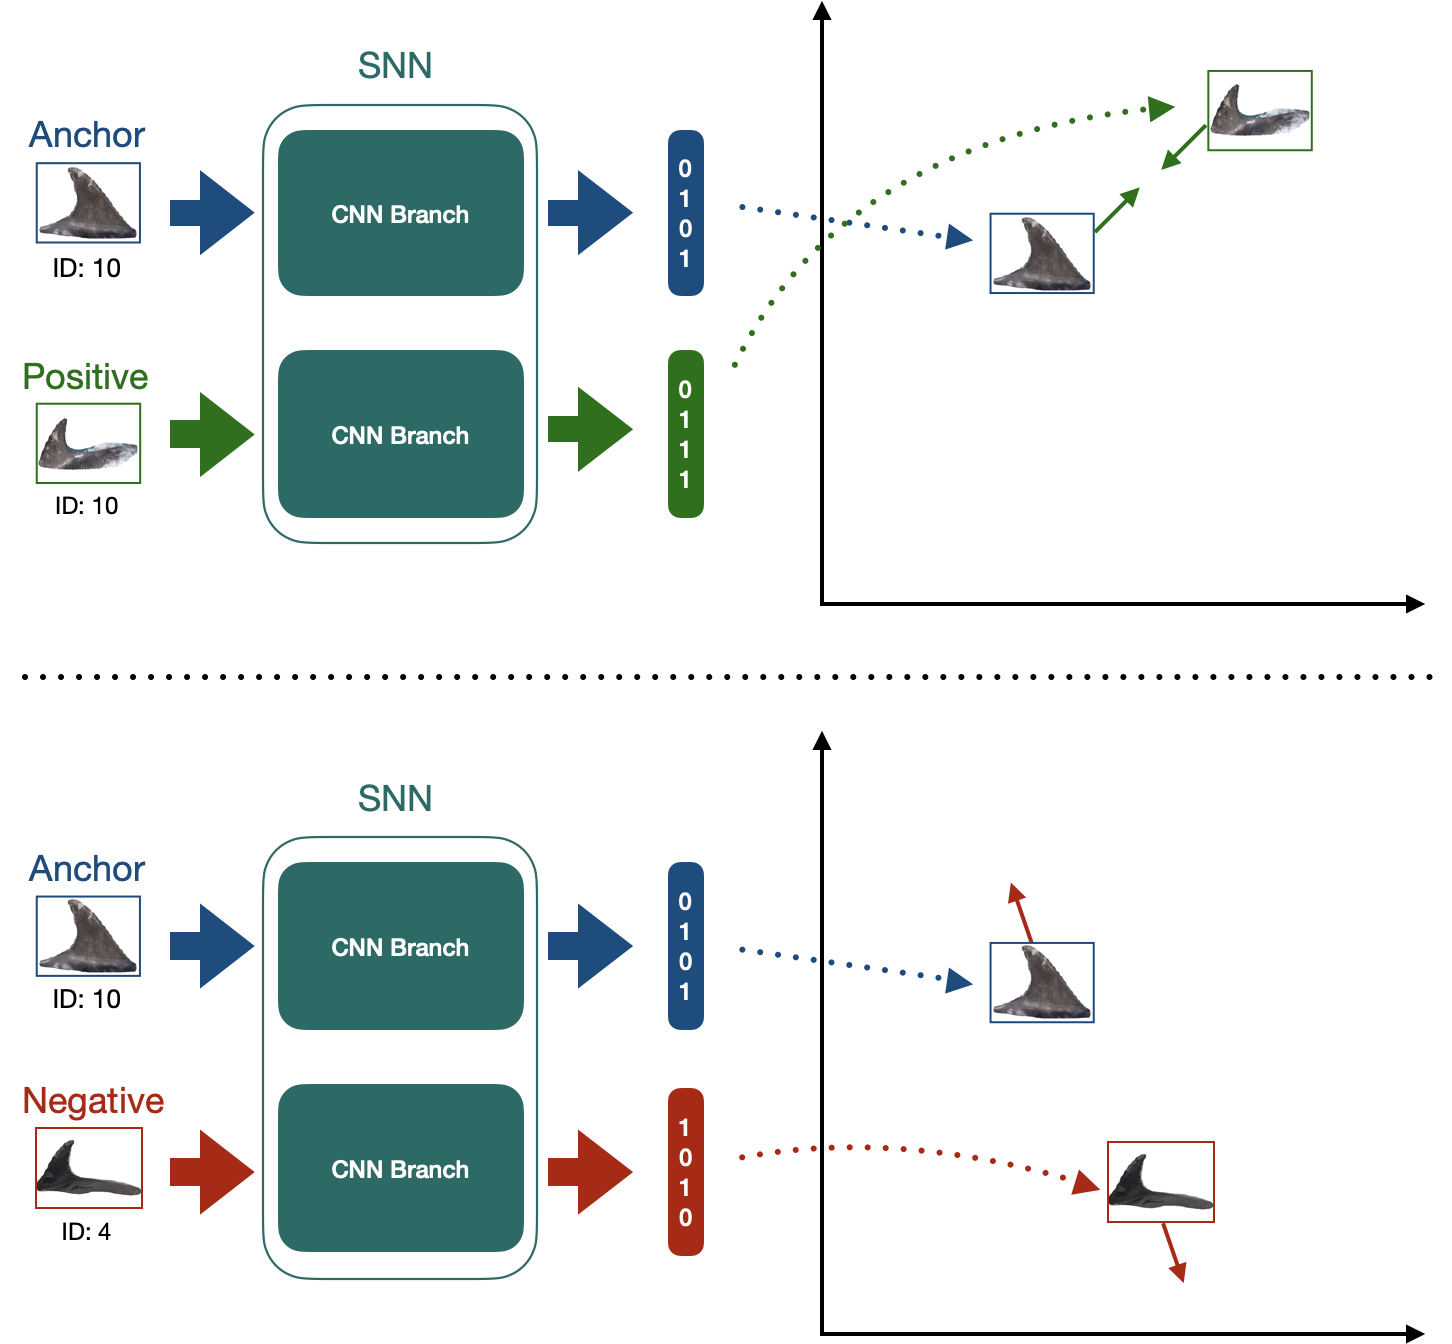
\includegraphics[scale=0.5]{Chapter6/figs/pairwise_ranking_loss_faces-updated.png}
	\end{center}
	\caption[SNN optimisation using Pairwise Ranking Loss.]{SNN optimisation using Pairwise Ranking Loss. Each input is passed to a branch of the SNN and an embedding is produced. These embeddings are used to optimise future embedding generation, aiming to either pull the Anchor and Positive together or push the Anchor and Negative apart.}
	\label{fig:pairwise_ranking_loss_faces}
\end{figure}

Using these two input types Pairwise Ranking Loss can be used to optimise in such a way that the model learns to produce embeddings with a small distance between Anchors and Positives, and a large distance between Anchors and Negatives. Mathematically Pairwise Ranking Loss can be defined using Equation \ref{eq:pairwiseLoss}:

\begin{equation}
	\label{eq:pairwiseLoss}
	L =
		\begin{cases}
			D(A, P) & \text{if Positive Pair}\\
			max(0, m - D(A, N)) & \text{if Negative Pair}\\
		\end{cases}       
\end{equation}

\noindent Where $L$ is the loss, $D(A, P)$ is the distance between the Anchor and the Positive, and $D(A, N)$ is the distance between the Anchor and the Negative. When optimising for Positive Pairs the loss function will only ever return 0 when the distance between the Anchor and the Positive is 0, ensuring these embeddings are nearly always pulled closer. When optimising for Negative Pairs, the loss function will return 0 when the distance between the Anchor and the Negative is greater than some margin $m$. As such, a weight update is not performed when the distance between the Anchor and the Negative is sufficiently large.

\subsubsection{Triplet Ranking Loss}\label{ch:ID,sec:SNNBackground,sub:lossFunction,subsub:Triplet}

One of the main problems presented by Pairwise Ranking Loss is the issue of model collapse, occurring after a large amount of Positive Pair optimisations. In this scenario, the distance between Anchors and Positives is pushed so close together in the latent space as to produce the same embedding. This can in turn affect the model's ability to understand variation in input and similarity scoring. 

Triplet Ranking Loss aims to avoid this issue by training on triplets of data points rather than pairs, with each triplet containing an Anchor, a Positive, and a Negative. SNNs which make use of Triplet Ranking Loss are often named Triplet Networks in the literature \cite{hoffer_deep_2018}, however the only difference between the structure of an SNN using Pairwise Ranking Loss or Triplet Ranking Loss is the number of branches -- two or three respectively. 

\begin{figure}
	\begin{center}
		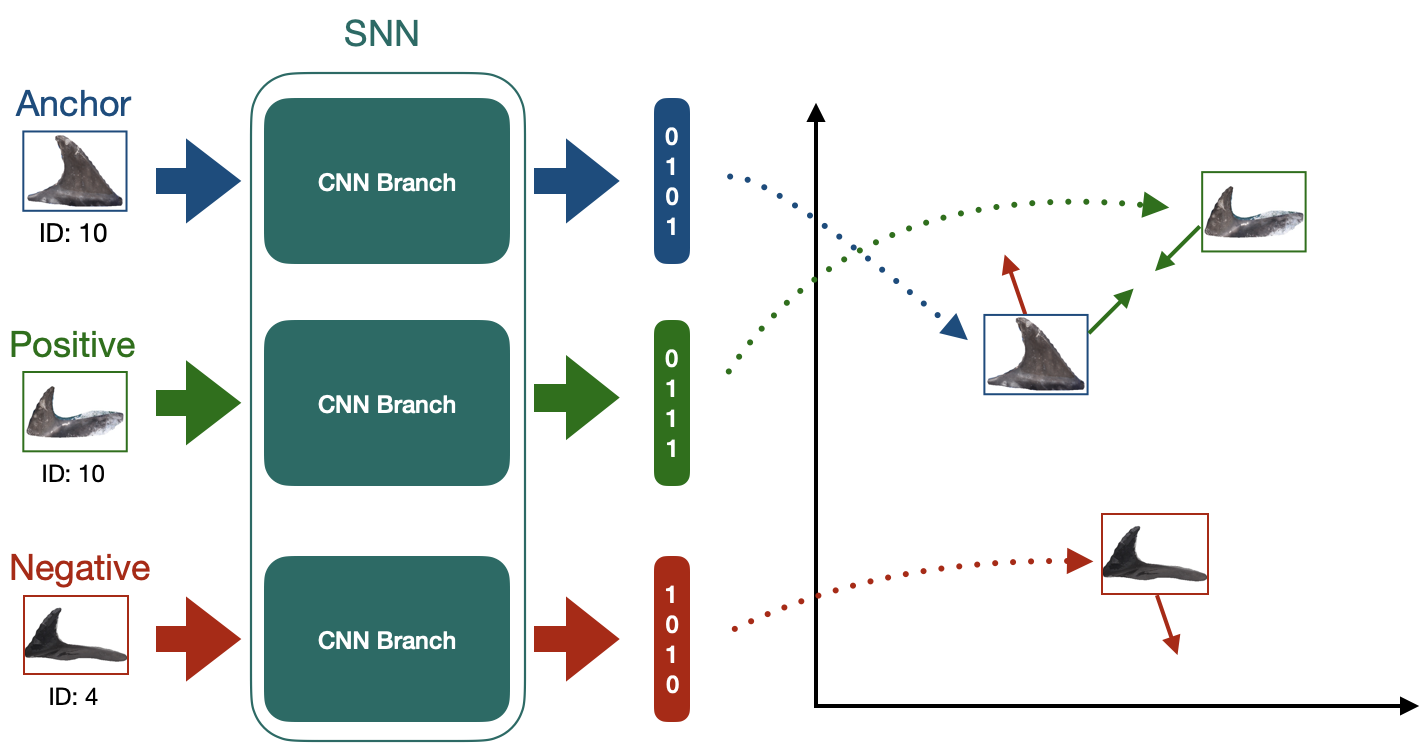
\includegraphics[scale=0.5]{Chapter6/figs/triplet-loss-eg-updated.png}
	\end{center}
	\caption[SNN optimisation using Triplet Ranking Loss.]{SNN optimisation using Triplet Ranking Loss. Each input is passed to a branch of the SNN and an embedding is produced. These embeddings are used to optimise future embedding generation, aiming to both pull the Anchor and Positive together whilst pushing the Anchor and Negative apart.}
	\label{fig:triplet-loss-eg}
\end{figure}

Just like with Pairwise Ranking Loss, Triplet Ranking Loss takes as input the generated embeddings for each branch and optimises to pull the Anchor and Positive close whilst pushing the Negative away, as visualised in Figure \ref{fig:triplet-loss-eg}. Optimisation is performed using Equation \ref{eq:tripletLoss}:

\begin{equation}
	\label{eq:tripletLoss}
	L = max(0, D(A, P) - D(A, N) + m)
\end{equation}

By utilising a triplet, the loss function evaluates to 0 when $D(A, N) > D(A, P) + m$. This occurs only when the triplet contains examples the model is already well trained on and no further optimisations can be gained. By enforcing $m$, where typically $m = 0.2$ thanks to work by Schroff \textit{et al.} \cite{schroff_facenet_2015}, the function ensures embedding variation between distinct inputs thus allowing for a similarity score to be computed between the Anchor and the Positive in all cases. Thanks to the advantages of Triplet Ranking Loss over its Pairwise counterpart, the decision was made to make use of this loss function and train an SNN with three branches. Further, Triplet Ranking Loss has been shown to perform well on individual identification tasks in both humans \cite{hermans_defense_2017} and animals \cite{vetrova_hidden_2018}, providing evidence to support its use for training a most likely catalogue matcher.

\subsection{Semi-Hard Triplet Mining}\label{ch:ID,sec:SNNBackground,sub:SemiHardTripletMining}

When training a model, care should be taken to ensure learning occurs at every step. When using Triplet Ranking Loss however, learning does not occur during training steps where the loss evaluates to 0, such as when $D(A, N) > D(A, P) + m$. Negatives provided should be sufficiently difficult such that the triplet allows the loss to evaluate to a non-zero value, ensuring the model learns and the training step is not wasted. However care should also be taken so as not to provide the model with triplets that are too difficult, as this will increase optimisation and thus overall training time. 

This leads to somewhat of a Goldilocks problem. Triplets must be not so soft as to prevent learning, but not so hard as to dramatically increase training time. Semi-Hard Triplet Mining aims to fix this problem, providing triplets which are \textit{just right}. A triplet, $T$, is defined using Equation \ref{eq:triplets}:

\begin{equation}
	\label{eq:triplets}
	T =
	\begin{cases}
		D(A, P) + m < D(A, N) & \text{if Easy}\\
		D(A, N) < D(A, P) & \text{if Hard}\\
		D(A, P) < D(A, N) < D(A, P) + m & \text{if Semi-Hard}
	\end{cases}       
\end{equation}

The goal of Semi-Hard Triplet Mining is to locate as many Semi-Hard triplets from the training set as possible. These are triplets whereby the loss still evaluates to a positive value however the Anchor is closer to the Positive than the Negative when plotted in the latent space, as seen in Figure \ref{fig:semi-hard-triplet-mining}. This allows for fast training whilst still providing enough triplet difficulty for the model to learn during training. 

\begin{figure}
	\begin{center}
		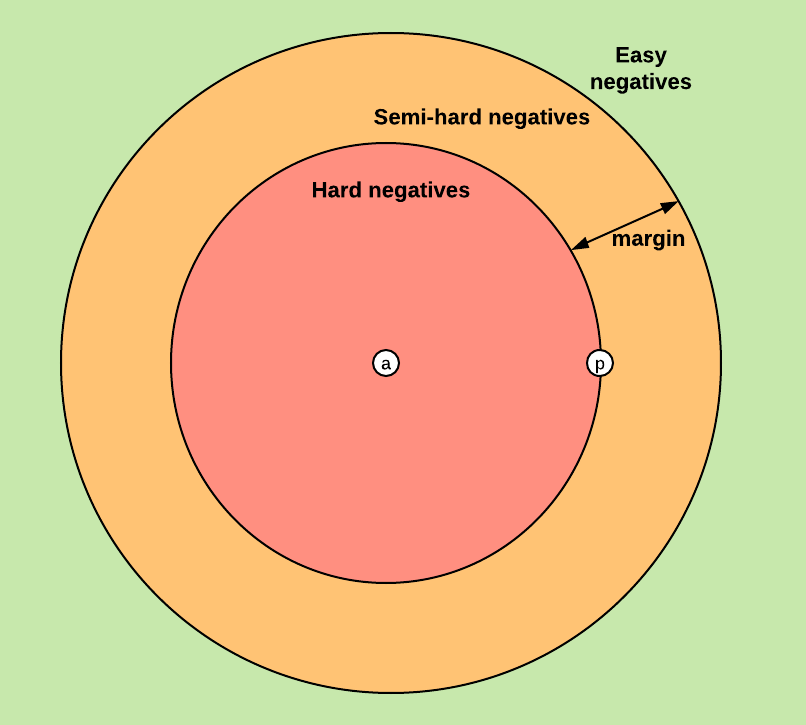
\includegraphics[scale=0.7]{Chapter6/figs/semi-hard-triplet-mining.png}
	\end{center}
	\caption[A visualisation of the areas in the latent space where Easy, Hard, and Semi-Hard triplets can occur.]{A visualisation of the areas in the latent space where Easy, Hard, and Semi-Hard triplets can occur, where $a$ is the location of the Anchor and $p$ is the location of the Positive. Image from \cite{moindrot_triplet_2018}.}
	\label{fig:semi-hard-triplet-mining}
\end{figure}

Finding, or mining, Semi-Hard triplets can be performed either Offline or Online. In Offline mining, the entire training set is converted into triplets before the training epoch occurs and those that fit the Semi-Hard definition are utilised. With Online mining, Semi-Hard triplets are generated on the fly as required. Generally, Online mining results in faster training when compared to Offline mining as this allows for the ability to update our definition of a Semi-Hard Triplet as training progresses.

\subsection{Class Prototyping}\label{ch:ID,sec:SNNBackground,sub:prototypes}

After SNN training it is possible to obtain likely classifications for an input based on Euclidean distance measurements between the input's embedding and the previously generated embeddings when plotted into the latent space. If there is a large number of embeddings in the space however this can increase classification time, as the input's embedding must be checked against every other in the space. 

There are ways to reduce the time taken for this calculation to complete by reducing the number of distance measurements that occur. A naive approach would be to, for example, randomly select one embedding for each class and measure the distance between it and the input embedding such that the distance to each class is only measured once, vastly reducing the computation required for classification. This may only work however when the class embeddings are perfectly clustered in the latent space, which will likely not be the case when using real world data.

There may also be cases where embeddings are not clustered with their class, such as in Figure \ref{fig:naive-embedding-example} where an embedding of class \texttt{cross} has been generated such that it is surrounded by examples of class \texttt{square} -- far from the other \texttt{cross} examples. There is also a triangle in the top-right of the Figure which represents the embedding location of an unclassified inference image. 

 \begin{figure}[h]
	\begin{center}
		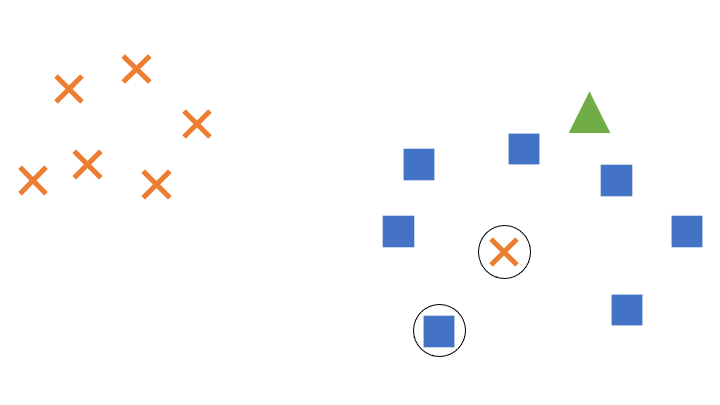
\includegraphics[scale=0.5]{Chapter6/figs/naive-embedding-example.png}
	\end{center}
	\caption{An example latent space with two classes (\texttt{cross} and \texttt{square}) alongside a triangle which represents the embedding location of an unclassified inference image. The two class examples selected for distance measurement to classify the triangle using the naive approach are circled.}
	\label{fig:naive-embedding-example}
\end{figure}

Using the naive approach to classify this triangle as either a \texttt{cross} or \texttt{square}, assuming the two randomly selected class embeddings are the ones circled in the Figure, then the triangle would be classified as an example of class \texttt{cross}. However, looking at the space globally is is clear the triangle should more likely be classified as a \texttt{square}; the chosen \texttt{cross} is simply an outlier. By selecting embeddings to measure from, the risk of outliers skewing the distance measurement, and thus the final classification, increases. This risk can be mitigated through the use of class prototypes -- generalised embeddings generated from the median embedding for all examples of each class. By making use of prototypes, the effect of outliers during classification is reduced.

Figure \ref{fig:prototype-embedding-example} shows the same example two class latent space as before, however it now also displays the generated class prototypes $P_{\times}$ and $P_{\rule{0.8ex}{0.8ex}}$ respectively. If the distance measurement is performed using the prototypes, the triangle is now classified as a \texttt{square}, which is more likely given the construction of the global space.

\begin{figure}[h]
	\begin{center}
		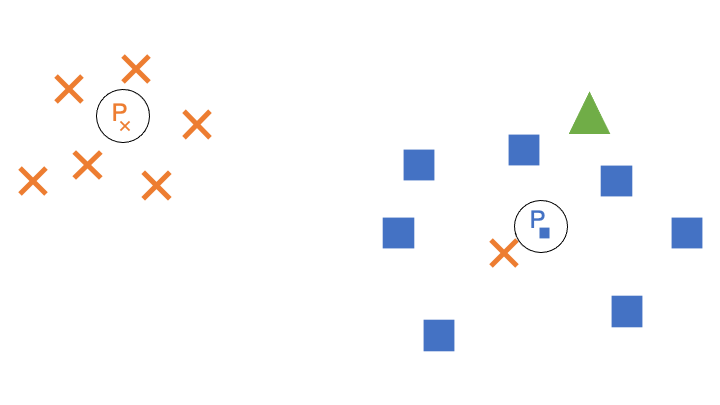
\includegraphics[scale=0.5]{Chapter6/figs/prototype-embedding-example.png}
	\end{center}
	\caption{An example latent space with two classes (\texttt{cross} and \texttt{square}) alongside a triangle which represents the embedding location of an unclassified inference image. The two class prototypes used to classify the triangle, $P_{\times}$ and $P_{\rule{0.8ex}{0.8ex}}$ respectively, are circled.}
	\label{fig:prototype-embedding-example}
\end{figure}

This method is not without its limitations either however. If all examples of the \texttt{cross} class formed a circle of radius 1 around the origin and all \texttt{square} examples formed a circle of radius 2, in both cases the class prototypes would be formed at the origin resulting in equal distance measurements. Although the chances of this are small, and these formations could be avoided using different hyperparameters or model architecture, it is important to be aware that this could happen when utilising prototypes. 

\subsection{Top-N Accuracy}\label{ch:ID,sec:SNNBackground,subsec:TopNAccuracy}

In coarse-grained computer vision tasks such as image classification, the effectiveness of a model is evaluated using, among other metrics, an accuracy score. Given an image in the test dataset, the model's class prediction for the image, defined as the class which has the highest probability assigned to it, is compared against the ground truth class label. If the predicted and ground truth classes are the same, the model is correct and is operating as intended. Performing this process iteratively over all images in the test dataset provides an accuracy score, often written as a percentage denoting how many test images the model classified correctly.

Due to the low inter-class differences between the classes in a fine-grained dataset however, the same model may struggle to consistently assign the highest probability to an image's ground truth. Using the coarse-grained definition of accuracy, this model may now perform poorly. However for certain tasks, such as most likely catalogue matching, the model may be considered effective simply if it is able to reduce the range of classification possibilities.

As such, the top-$N$ accuracy metric is often utilised for fine-grained classification tasks \cite{yang_large-scale_2015, gao_towards_2021, brust_towards_2017}. Rather than only outputting the class with the highest probability, the model instead takes the $N$ highest probabilities, outputting its prediction as a list of possible values. If the ground truth class is contained within the list, the model is considered to be correct. 

For example, utilising top-10 accuracy the model would output the 10 highest probabilities for an image and would be considered correct if the ground truth label was within this list. Utilising top-1 accuracy would force the model to output a single prediction, which would be the same as utilising the standard accuracy definition. 

As the task of most likely catalogue matching is a fine-grained problem, developed SNNs are evaluated using the top-$N$ accuracy metric. Furthermore, as the goal of this work is to produce a system which aids researchers through the task of catalogue matching rather than fully replace them, it is beneficial for the SNNs to produce a list of predictions as this will greatly reduce the number of individuals the researcher needs to examine in order to be confident of a match.

\section{Siamese Neural Network Development}\label{ch:ID,sec:SNNDevelopment}

The following sections detail the creation of the SNN-based catalogue matcher. Figure \ref{fig:pipeline-SNN} highlights where in the system pipeline this model will be placed.

\begin{figure}[!h]
	\begin{center}
		\includegraphics[width=\linewidth]{Chapter6/figs/pipeline-SNN.png}
	\end{center}
	\caption[The high level pipeline overview, shown in Figure \ref{fig:pipeline}, with the SNN component highlighted.]{The high level pipeline overview, shown in Figure \ref{fig:pipeline}, with the SNN component highlighted. It is this part of the pipeline that will be discussed in the following sections.}
	\label{fig:pipeline-SNN}
\end{figure}

Two backbone architectures were tested during SNN development. The first of these was the architecture defined in Vetrova \textit{et al.} \cite{vetrova_hidden_2018}, hereafter denoted as VarvaraNet. This was utilised to examine whether a network which is proven capable at species identification is also able to perform well for the task of individual identification. The second was a custom architecture consisting of a Convolutional layer, a Dropout layer, a PReLU layer, and a MaxPool layer (stride = 2). This network was utilised to examine whether a more basic backbone would be capable of performing well given the fine-grained, few-shot nature of the task. This architecture is hereafter denoted as EmbeddingNet. To aid development, this work made use of Adam Bielski's PyTorch implementation of SNNs\footnote{\textit{Siamese and triplet learning with online pair/triplet mining} repository by Adam Bielski: \href{https://github.com/adambielski/siamese-triplet}{github.com/adambielski/siamese-triplet}}.

\subsection{Hyperparameter Tuning Via Bayesian Optimisation }\label{ch:ID,sec:SNNDevelopment,sub:Optuna}

Like all models, SNNs have multiple hyperparameters which must be tuned. As such, work began to select which hyperparameters should be tuned and how. Since developing the Mask R-CNN fin detector, discussed in Chapter \ref{ch:cetDet}, the area of hyperparameter optimisation has advanced considerably. Multiple frameworks now exist which take a Bayesian approach to finding the optimal hyperparameter values. Unlike optimisation through a Grid Search whereby all combinations of user-defined hyperparameter values are evaluated (see Section \ref{ch:cetDet,sec:ModelSelection,sub:HyperparameterTuning} for an example of this), with Bayesian Optimisation the user only needs to define the upper and lower bounds for each hyperparameter. The search space is then explored using a probabilistic methodology, locating the optimal set of hyperparameters within the ranges provided. This speeds up the optimisation process as values unlikely to yield promising results are ignored. As such, a larger number of hyperparameters can be optimised when compared to a Grid Search, and this can be achieved in a smaller amount of time. 

The Optuna framework \cite{akiba_optuna_2019}  was utilised to facilitate hyperparameter tuning through Bayesian optimisation. Whilst Optuna allows users to make use of custom optimisation algorithms, this work specifically made use of the built-in Tree-structured Parzen Estimator (TPE)\nomenclature[z-TPE]{TPE}{Tree-structured Parzen Estimator}	 algorithm. Optuna performs optimisation iteratively. This means that, for each iteration and for each hyperparameter, TPE fits one Gaussian Mixture Model to the set of hyperparameter values, $x$, associated with the current optimal values, $l(x)$, and another to the remaining hyperparameter values, $g(x)$. Optimal values for each iteration are selected by maximising the ratio $l(x)/g(x)$, with the final trial producing the current optimal hyperparameter values. For a more in-depth discussion of TPE, see Bergstra \textit{et al.} \cite{bergstra_algorithms_2011}.

Through Optuna, TPE was utilised to set the learning rate to a \texttt{log uniform} value between $1\times10^{-6}$ and $1\times10^{-3}$, for use with either the SGD or Adam optimiser.  Weight decay was set to a \texttt{log uniform} value between $1\times10^{-6}$ and $1\times10^{-1}$. Step size was set to an \texttt{int} value between 5 and 10, with the $\gamma$ value for this set to a \texttt{log uniform} between $1\times10^{-3}$ and $1\times10^{-1}$. The margin, $m$, defined in the Triplet Ranking Loss (see Equation \ref{eq:tripletLoss}) was set to a \texttt{log uniform} value between 0.1 and 1.0. The final embedding layer was tuned to produce an \texttt{int} value between 16 and 128.

Optimisation of the number of network blocks was also examined. For VarvaraNet a block consisted of a Convolutional layer, a MaxPool layer (stride = 2), a ReLU layer, and a Dropout layer. For EmbeddingNet a block consisted of a Convolutional layer, a Dropout layer, a PReLU layer, and a MaxPool layer (stride = 2). During searching, the number of blocks was treated as a hyperparameter optimising for an \texttt{int} between 1 and 5 blocks. The size of the initial Convolutional layer was also tuned, searching for an optimal \texttt{int} value between 16 and 100. Subsequent layers were double the size of the previous. Dropout was set to search for a \texttt{log uniform} value between 0.1 and 0.7. The kernel size of the initial Convolutional layer was set to a \texttt{categorical} value of either 5, 6, 7, or 8 with subsequent layers set according to $max(1, k - 2)$ where $k$ is the kernel size of the previous Convolutional layer.

\subsection{Data Augmentation Strategy}\label{ch:ID,sec:SNNDevelopment,sub:DataAugmentation}

The use of data augmentation was also examined. The decision was made to reduce the variety of augmentations performed compared to Mask R-CNN development, as discussed in Section \ref{ch:cetDet,sec:initialTesting,sub:dataaugmentation}. At this stage in the pipeline the data seen by the SNN has been post-processed, thus it would not be realistic to utilise an aggressive data augmentation strategy over the NDD AU SMRU dataset. Further, an aggressive strategy may obscure the identifying markers present on the fins too much for meaningful training to occur. 

The first strategy, Colour Jitter, randomly perturbs the input images' brightness by a factor of between 0.8 and 1.2, contrast by a factor of between 0.8 and 1.2, saturation by a factor of 0.9 and 1.1, and hue by a factor of -0.1 and 0.1. The second, Perspective Shift, randomly distorts the input image's perspective by a factor of 0.5. The third, Greyscale, converted the three-channel RGB input image into a single-channel greyscale image. Tests examining combinations of these strategies were also examined, such as augmenting with both Colour Jitter and Perspective Shift. Note that Greyscale cannot be combined with Colour Jitter due to the reduction in colour channels required. 

\section{Siamese Neural Network Model Selection}\label{ch:ID,sec:ModelSelection}

Models with both VarvaraNet and EmbeddingNet architectures were trained for the task of most likely catalogue matching using the NDD AU SMRU dataset and the data augmentation strategies defined in Section \ref{ch:ID,sec:SNNDevelopment,sub:DataAugmentation}. Hyperparameter optimisation was performed for each architecture-augmentation combination, as each architecture and augmentation strategy may influence the optimal hyperparameters for the model.

To perform hyperparameter tuning through Bayesian optimisation, both a train and validation set is required, with the former utilised to train the selected architecture using the current iteration's selected hyperparameters and the latter utilised to evaluate how well this model performs against unseen data -- acting like the test set for each iteration. As such the dataset was first divided randomly using an 80-20 train-test split. The train set was then divided randomly further for optimisation, with 30\% of the train set held for validation, resulting in an overall 56-24-20 train-validation-test split.

Whilst the train and validation splits may feel unnatural (a 56-24 split is not common in the literature), splitting in this way ensures that a high variety of Semi-Hard triplets can be generated at all points in the training process. To further aid this, before splitting the dataset was filtered to remove any classes which contained fewer than six example images. Performing this step has the added benefit of allowing some individuals to be held back to examine the SNN's ability to flag those it has not been trained to recognise, as these can be treated as uncatalogued individuals. 

Once the final optimal hyperparameters had been located using Bayesian optimisation, the train and validation sets were recombined and used to train the selected architecture from scratch using the located hyperparameters, alongside the selected data augmentation strategy. Once trained, the model was then evaluated using the test set. 

\begin{table}[h]
	\centering
	\begin{tabular}{ccccc}
		\hline
		\multirow{2}{*}{\textbf{\begin{tabular}[c]{@{}c@{}}Model\\ Backbone\end{tabular}}} & \multirow{2}{*}{\textbf{\begin{tabular}[c]{@{}c@{}}Data Augmentation\\ Strategy\end{tabular}}} & \multicolumn{3}{c}{\textbf{Accuracy (\%)}}             \\ \cline{3-5} 
		&                                                                                                & \textbf{Top-1}     & \textbf{Top-5}     & \textbf{Top-10}    \\ \hline
		EmbeddingNet                                                                       & Greyscale                                                                                      & 30.69          & 58.13          & 75.00          \\
		VarvaraNet                                                                         & Greyscale                                                                                      & 42.07          & 62.20          & 74.80          \\
		EmbeddingNet                                                                       & \begin{tabular}[c]{@{}c@{}}Greyscale \&\\ Perspective Shift\end{tabular}                        & 35.57          & 51.02          & 68.30          \\
		VarvaraNet                                                                         & \begin{tabular}[c]{@{}c@{}}Greyscale \&\\ Perspective Shift\end{tabular}                        & 38.82          & 62.60          & 77.64          \\
		EmbeddingNet                                                                       & None                                                                                           & 39.63          & 66.46          & 79.06          \\
		\textbf{VarvaraNet}                                                                & \textbf{None}                                                                                  & \textbf{40.85} & \textbf{68.90} & \textbf{83.13} \\
		EmbeddingNet                                                                       & Colour Jitter                                                                                  & 28.05          & 50.00          & 66.67          \\
		VarvaraNet                                                                         & Colour Jitter                                                                                  & 38.82          & 61.18          & 76.83          \\
		EmbeddingNet                                                                       & Perspective Shift                                                                              & 22.36          & 47.15          & 65.24          \\
		VarvaraNet                                                                         & Perspective Shift                                                                              & 23.17          & 51.22          & 73.58          \\
		EmbeddingNet                                                                       & \begin{tabular}[t]{@{}c@{}}Perspective Shift \&\\ Colour Jitter\end{tabular}                    & 30.69          & 53.25          & 68.49          \\
		VarvaraNet                                                                         & \begin{tabular}[t]{@{}c@{}}Perspective Shift \&\\ Colour Jitter\end{tabular}                    & 40.04          & 61.18          & 78.46          \\ \hline
	\end{tabular}
	\caption[Results of SNN training for the task of most likely catalogue matching on the NDD AU SMRU dataset.]{Results of SNN training for the task of most likely catalogue matching on the NDD AU SMRU dataset. The model chosen for use is highlighted in bold.}
	\label{fig:NDDAUSMRU-SNN-model-accuracies}
\end{table}

Table \ref{fig:NDDAUSMRU-SNN-model-accuracies} shows the results of training an SNN to perform most likely catalogue matching on the NDD AU SMRU dataset. Each model trained is evaluated using top-1, top-5, and top-10 accuracies. As can be seen, the best performing model is a VarvaraNet trained without the use of any data augmentation. This model achieves the highest test set accuracy at all evaluated metric thresholds, achieving 40.85\% top-1, 68.90\% top-5, and 83.13\% top-10 accuracies. These results provide evidence that SNNs are capable of fine-grained, few-shot individual level identification. If the model was deployed into production and utilised by cetacean researchers, then these levels of accuracy would vastly reduce the search space required to perform most likely catalogue matching.

On the whole, it is the case that models using an EmbeddingNet backbone perform worse than those using a VarvaraNet backbone, even when utilising the same data augmentation strategies. Furthermore it can be seen that, in general, the data augmentation strategy chosen for training has little effect on final model performance against the test set as evidenced by the lack of variation in accuracy metrics between models when trained using different strategies. This is especially interesting with regards to the greyscale augmentation as whilst there has been a drop in accuracy when compared to the best performing model this is only slight. However, this does suggest that a reduction in colour channel leads to some information loss. The fact that the best performing model is one which makes use of no data augmentations may suggest that even strategies which only perturb the input slightly still have a negative effect on the model's ability to extract identifying information. 

\subsection{An Evaluation of Optimal Model Hyperparameters}\label{ch:ID,sec:ModelSelection,subsec:paramEval}

The optimal SNN hyperparameters chosen through Bayesian optimisation for each architecture-augmentation training run can be seen in Table \ref{tab:optunaBestParamsPerSNN}. Of the models trained, 83\% of them use Adam \cite{kingma_adam:_2014} as an optimiser, including the best performing model (VarvaraNet without data augmentation). This aligns with the belief within deep learning research that Adam will often provide optimal model training \cite{karpathy_peek_2017}.

\begin{table}[!t]
	\centering
	\resizebox{!}{.55\height}{
		\small
		\begin{tabular}{ccccccccccccc}
			\hline\vspace{0.01cm}
			\textbf{\begin{tabular}[c]{@{}c@{}}Model\\Backbone\end{tabular}} & \textbf{\begin{tabular}[c]{@{}c@{}}Data\\Augmentation\\Strategy\end{tabular}} & \textbf{\begin{tabular}[c]{@{}c@{}}Network\\Blocks\end{tabular}} & \textbf{\begin{tabular}[c]{@{}c@{}}Initial\\Convolutional\\Layer\\Size\end{tabular}} & \textbf{\begin{tabular}[c]{@{}c@{}}Initial\\Convolutional\\Layer\\Kernel\\Size\end{tabular}} & \textbf{Dropout} & \textbf{\begin{tabular}[c]{@{}c@{}}Learning\\Rate\end{tabular}} & \textbf{Optimiser} & \multicolumn{1}{c}{\textbf{\begin{tabular}[c]{@{}c@{}}Weight\\Decay\end{tabular}}} & \multicolumn{1}{c}{\textbf{\begin{tabular}[c]{@{}c@{}}Step\\Size\end{tabular}}} & \textbf{$\gamma$} & \textbf{\begin{tabular}[c]{@{}c@{}}Embedding\\Size\end{tabular}} & \textbf{\begin{tabular}[c]{@{}c@{}}Triplet\\Ranking\\Loss\\Margin\end{tabular}} \\ \hline
			EmbeddingNet                                                       & Greyscale                                                                        & 5                                                                 & 37                                                                                     & 8                                                                                             & 0.677            & $2.578\times10^{-6}$                                                          & Adam               & $5.008\times10^{-5}$                                                                            & 6                                                                                 & 0.048             & 120                                                               & 0.551                                                                             \\
			VarvaraNet                                                         & Greyscale                                                                        & 2                                                                 & 60                                                                                     & 5                                                                                             & 0.358            & $1.031\times10^{-4}$                                                          & Adam               & $3.680\times10^{-5}$                                                                             & 5                                                                                 & 0.036             & 17                                                                & 0.863                                                                             \\
			EmbeddingNet                                                       & \begin{tabular}[t]{@{}c@{}}Greyscale \&\\ Perspective Shift\end{tabular}         & 5                                                                 & 26                                                                                     & 7                                                                                             & 0.261            & $1.214\times10^{-4}$                                                          & Adam               & $8.364\times10^{-3}$                                                                            & 10                                                                                & 0.081             & 65                                                                & 0.684                                                                             \\
			VarvaraNet                                                         & \begin{tabular}[t]{@{}c@{}}Greyscale \&\\ Perspective Shift\end{tabular}         & 5                                                                 & 62                                                                                     & 5                                                                                             & 0.269            & $1.817\times10^{-6}$                                                           & Adam               & $1.954\times10^{-4}$                                                                             & 5                                                                                 & 0.030             & 91                                                                & 0.860                                                                             \\
			EmbeddingNet                                                       & None                                                                             & 3                                                                 & 29                                                                                     & 7                                                                                             & 0.242            & $2.835\times10^{-5}$                                                          & Adam               & $9.106\times10^{-3}$                                                                             & 8                                                                                 & 0.001             & 69                                                                & 0.758                                                                             \\
			\textbf{VarvaraNet}                                                         & \textbf{None}                                                                             & \textbf{2}                                                                 & \textbf{59}                                                                                     & \textbf{6}                                                                                             & \textbf{0.169}            & $\mathbf{7.253\times10^{-6}}$                                                          & \textbf{Adam}               & $\mathbf{4.338\times10^{-2}}$                                                                             & \textbf{10}                                                                                & \textbf{0.012}             & \textbf{106}                                                               & \textbf{0.796}                                                                            \\
			EmbeddingNet                                                       & Colour Jitter                                                                    & 5                                                                 & 44                                                                                     & 6                                                                                             & 0.197            & $1.876\times10^{-5}$                                                          & Adam               & $3.567\times10^{-6}$                                                                             & 6                                                                                 & 0.011             & 40                                                                & 0.436                                                                             \\
			VarvaraNet                                                         & Colour Jitter                                                                    & 3                                                                 & 38                                                                                     & 5                                                                                             & 0.684            & $9.251\times10^{-4}$                                                          & SGD                & $7.512\times10^{-4}$                                                                             & 5                                                                                 & 0.004             & 90                                                                & 0.281                                                                             \\
			EmbeddingNet                                                       & Perspective Shift                                                                & 5                                                                 & 42                                                                                     & 6                                                                                             & 0.120            & $1.653\times10^{-5}$                                                          & Adam               & $3.256\times10^{-3}$                                                                             & 5                                                                                 & 0.014             & 60                                                                & 0.273                                                                             \\
			VarvaraNet                                                         & Perspective Shift                                                                & 1                                                                 & 45                                                                                     & 6                                                                                             & 0.447            & $2.890\times10^{-4}$                                                          & Adam               & $4.458\times10^{-4}$                                                                             & 6                                                                                 & 0.004             & 24                                                                & 0.635                                                                             \\
			EmbeddingNet                                                       & \begin{tabular}[t]{@{}c@{}}Colour Jitter \&\\ Perspective Shift\end{tabular}     & 3                                                                 & 28                                                                                     & 6                                                                                             & 0.559            & $1.348\times10^{-6}$                                                          & Adam               & $1.608\times10^{-5}$                                                                             & 5                                                                                 & 0.073             & 51                                                                & 0.458                                                                             \\
			VarvaraNet                                                         & \begin{tabular}[t]{@{}c@{}}Colour Jitter \& \\ Perspective Shift\end{tabular}    & 2                                                                 & 35                                                                                     & 5                                                                                             & 0.286            & $4.093\times10^{-4}$                                                          & SGD                & $5.352\times10^{-4}$                                                                             & 9                                                                                 & 0.068             & 28                                                                & 0.826                       \\
			\bottomrule                                                      
	\end{tabular}}
	\caption[Optimal SNN hyperparameters for each architecture-augmentation combination located using Bayesian optimisation over 100 iterations.]{Optimal SNN hyperparameters for each architecture-augmentation combination located using Bayesian optimisation over 100 iterations. Results given to 3 decimal places where applicable. The model chosen for use is highlighted in bold.}
	\label{tab:optunaBestParamsPerSNN}
\end{table}

 Furthermore, in general the best results are achieved when utilising a low probability of dropout. This suggests that the models are not overfitting even with relatively small amounts of training data, which may be due to the low inter-class, high intra-class differences present in the dataset, as seen in Figure \ref{fig:segmented-ndd20-example}.
 
 Interestingly it is also the case that all hyperparameter optimisation runs, regardless of architecture or data augmentation strategy, settle on a Triplet Ranking Loss margin above 0.2, the value commonly used as a default for this hyperparameter thanks to work by Schroff \textit{et al.} \cite{schroff_facenet_2015}. There is a high deviation in margin value between the models, which may suggest that the use of 0.2 in all cases by default will not lead to optimal results.
 
 One important takeaway from the use of Bayesian optimisation techniques is that for some hyperparameters that require a continuous input, such as learning rate or weight decay, the optimal value may be one which would likely not be selected by a human when performing a Grid Search. This highlights the effectiveness of Bayesian optimisation over a Grid Search as, whilst the difference between a learning rate of $2\times10^{-6}$ selected during a Grid Search and $2.578\times10^{-6}$ selected by Bayesian optimisation, may only be a few percentage points increase in test set accuracy, this still results in an overall more generalisable model. 
 
\subsection{NDD AU SMRU Uncatalogued Individual Thresholding}\label{ch:ID,sec:ModelSelection,subsec:UncataloguedIndividualThresholding}

Further evaluation was performed to examine the best performing model's ability to flag uncatalogued individuals to the user. Before training, some classes from the NDD AU SMRU dataset were removed. As these are classes which have not yet been seen by the model, they can be utilised as if they were uncatalogued individuals.

\subsubsection{Thresholding via Class Prototypes}\label{ch:ID,sec:ModelSelection,subsec:UncataloguedIndividualThresholding,subsub:prototypes}

When an image is passed through the SNN its most likely catalogue matches are generated using the Euclidean distance between it and the available class prototypes. By clustering individuals together in the latent space based on embedding similarity and comparing new images using Euclidean distance to the generated class prototypes, the system can flag potentially previously uncatalogued individuals to the researcher - assuming the model has learnt to generate well defined class clusters. 

New individuals who have entered the catalogue's geographical survey area (e.g. through migration or birth) will thus have numeric representations which plot them into their own distinct location in the latent space, resulting in large Euclidean distances between that location and the existing photo-id catalogue prototypes. In order to flag potentially uncatalogued individuals, the use of a threshold was required. If the Euclidean distances between the input image and all class prototypes are above this threshold, then the input image is flagged to the user as a potentially uncatalogued individual. 

To decide on a threshold value for the NDD AU SMRU dataset, each image not utilised for SNN training was processed by the model and the distances between it and the class prototypes were empirically examined, in line with other works in this area \cite{battle_siamese_2022}. Through this, a threshold value of 4.0 was determined -- if the distance to the closest class prototype was above this value, then it is likely that the individual may be uncatalogued. An example of this can be seen in Figure \ref{fig:uncatalogued-individual-example-ndd-au-smru} (Top Right), which shows an example image of individual \texttt{3}, a class which was not included in the training of the model. As can be seen, the distance between the image's embedding and the closest class prototype is above the threshold, and thus the image has been flagged for manual review.

\begin{figure}[t]
	\begin{center}
		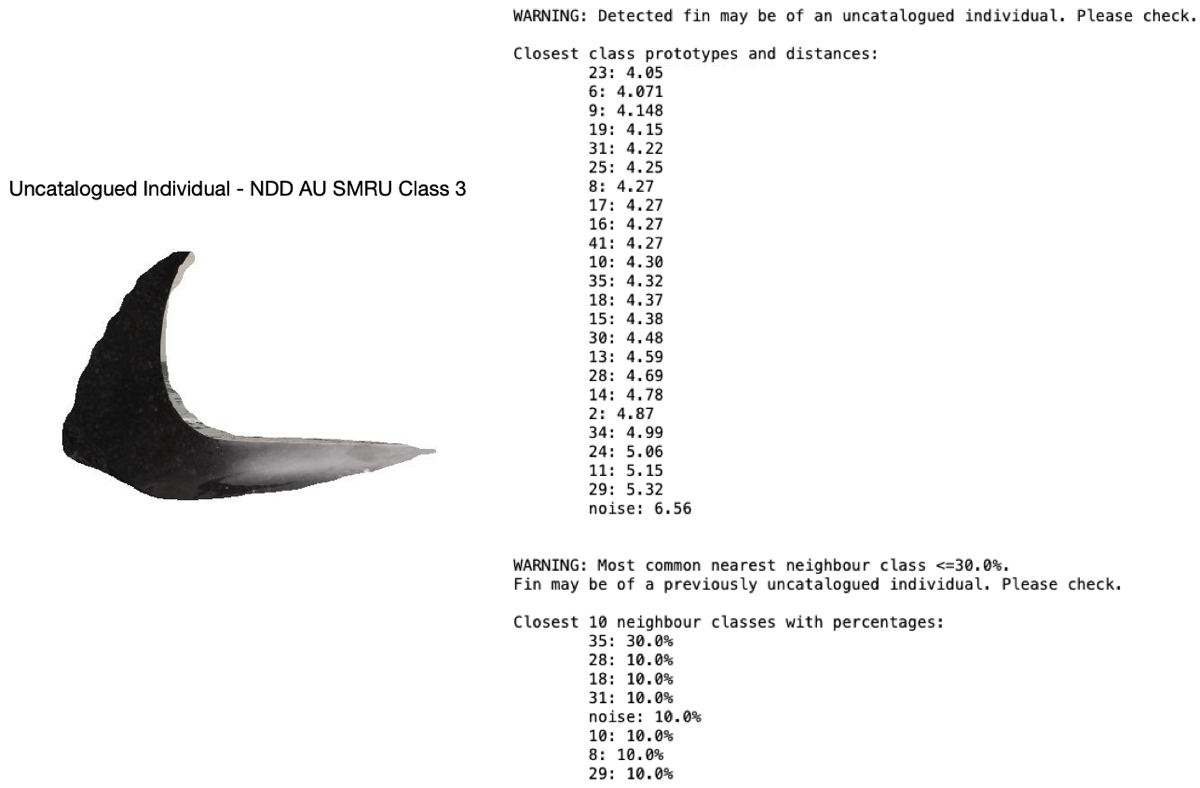
\includegraphics[width=\linewidth]{Chapter6/figs/uncatalogued-individual-example-ndd-au-smru-updated.png}
	\end{center}
	\caption[Example uncatalogued individual thresholding.]{Example uncatalogued individual thresholding. Left: the input image seen by the model, of class \texttt{3}. The model has not been trained using this class. Top Right: the resultant Euclidean distances between the input image's embedding and the existing class prototypes. As the distance to the closest prototype is above the threshold, the fin has been flagged for manual review. Bottom Right: uncertainty scores generated using K-Nearest Neighbours clustering. The model's most confident class is below the threshold, and thus the fin has been flagged for manual review.}
	\label{fig:uncatalogued-individual-example-ndd-au-smru}
\end{figure}

The use of class prototypes proved especially useful for determining noise. Through experimentation it was found that an image could be flagged as belonging to the noise class simply if the distance between the input image's embedding and the noise class prototype was the smallest, as seen in Figure \ref{fig:noise-individual-example-ndd-au-smru} (Top Right). This provides evidence to suggest that the model is capable of clustering examples of noise together well in the latent space, especially impressive as this class contains the highest intra-class variation as a result of containing all images of erroneous non-fin detections.

\begin{figure}[t]
	\begin{center}
		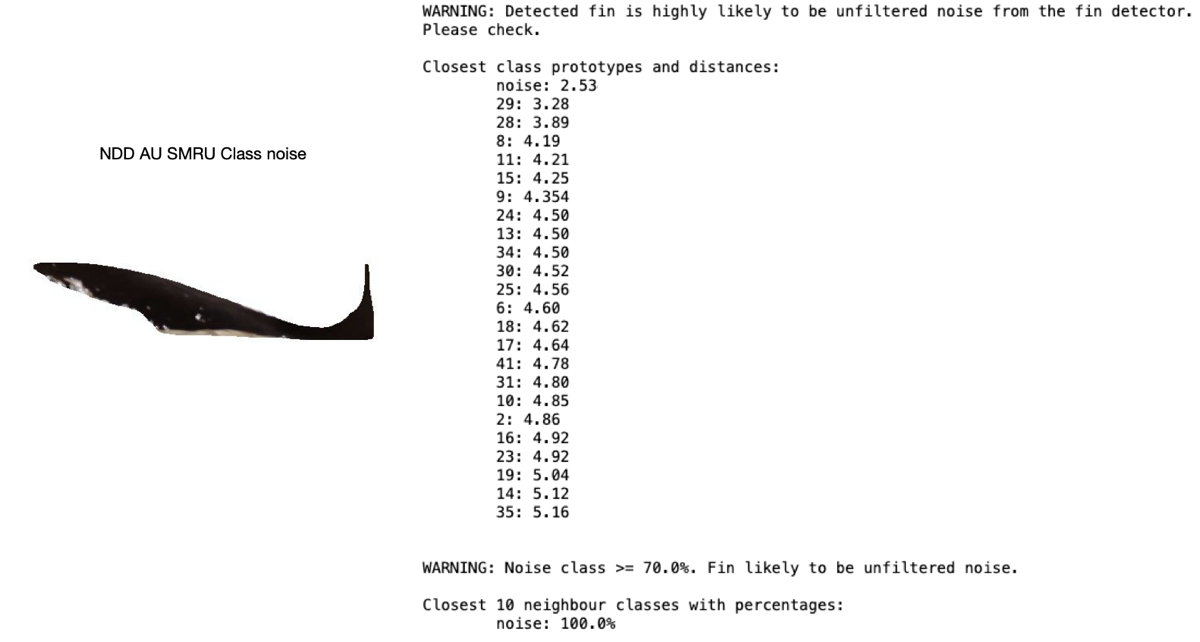
\includegraphics[width=\linewidth]{Chapter6/figs/noise-example-ndd-au-smru-updated.png}
	\end{center}
	\caption[Example noise thresholding.]{Example noise thresholding. Left: the input image seen by the model, of class \texttt{noise}. Top Right: the resultant Euclidean distances between the input image's embedding and the existing class prototypes. As the closest prototype is \texttt{noise}, the input has been flagged. Bottom Right: uncertainty scores generated using K-Nearest Neighbours clustering. The model's \texttt{noise} confidence is above the threshold, and thus the input has been flagged.}
	\label{fig:noise-individual-example-ndd-au-smru}
\end{figure}

\subsubsection{Thresholding via K-Nearest Neighbours}\label{ch:ID,sec:ModelSelection,subsec:UncataloguedIndividualThresholding,subsub:KNN}

 During experimentation it was found that when only utilising class prototypes, the model struggled to highlight uncatalogued individuals if some class clusters were spread over a large area in the latent space. To combat this, the use of K-Nearest Neighbours (KNN)\nomenclature[z-KNN]{KNN}{K-Nearest Neighbours} to flag potentially uncatalogued individuals was examined. KNN works by comparing each input image's embedding to the $K$ closest embeddings in the latent space, where $K$ is some user defined value. 
 
 If, for example, $K = 8$ then the closest eight embeddings to that of the input image are examined. If seven embeddings are of class \texttt{1} and one embedding is of class \texttt{2}, then we have an 88\% certainty that the input image is an example of class \texttt{2}. However, if the image is embedded and three of the closest eight embeddings are of class \texttt{1}, two are class \texttt{2}, one of class \texttt{3}, one of class \texttt{4}, and one of class \texttt{10}, then the uncertainty score for any classification of the input image would be high. This could then be flagged to the user. As such, the use of an uncertainty score allows for greater interpretability when compared to a similarity score based on distances between points in the latent space, especially for those without an understanding of the underlying concepts behind SNNs like cetacean researchers. 

During experimentation, it was found that setting $K = 10$ alongside an uncertainty threshold of 30\% allowed for the best chance of flagging uncatalogued individuals. If no class reached above 30\% certainty, this was flagged to the user as seen in Figure \ref{fig:uncatalogued-individual-example-ndd-au-smru} (Bottom Right). A noise threshold of 70\% was also enforced, whereby if the \texttt{noise} class confidence was above 70\% this would be flagged as seen in Figure \ref{fig:noise-individual-example-ndd-au-smru} (Bottom Right).

After experimentation with both methodologies, it was decided that utilising both class prototypes and KNN for flagging potentially uncatalogued individuals to the user would be best given the ability of the methodologies to complement one another. Whilst KNN allows for the production of an easily understandable metric for those without knowledge of the underlying processes of SNNs, the use of class prototypes provides a more nuanced, albeit latent space specific, metric. For all utilised uncatalogued images, 67.86\% were flagged using the above methodologies and threshold values. Both methods also allow for extra classes to be added to the latent space without the need for model fine-tuning or retraining. This means any uncatalogued individuals identified by the model can be added to the latent space to aid future identifications, alongside addition to the biological catalogue.

\subsection{Limitations of the Model}\label{ch:ID,sec:ModelSelection,sub:limitations}

As discussed in Section \ref{ch:ID,sec:ModelSelection}, the best performing SNN trained for most likely catalogue matching using the NDD AU SMRU dataset achieves 40.9\% top-1, 68.9\% top-5, and 83.1\% top-10 accuracies. Whilst these results are impressive given the fine-grained, few-shot nature of the task, it is important to also highlight the limitations of the approach. 

One limitation is the need to re-train the SNN for each new photo-id catalogue. As a result, initial manual curation must be performed before the proposed methodology can be applied. Evidence outlined in Section \ref{ch:ID,sec:ModelSelection,subsec:UncataloguedIndividualThresholding} suggests that, once trained, new classes can be added to the SNN with ease when a new individual is added to an existing catalogue -- however it is not yet clear whether this is the case in perpetuity or whether eventually the model is no longer able to generate meaningful clusters. The problem of drift, where model performance begins to degrade over time as the distribution of the data it receives naturally changes, is common with models once in production. It may be the case that as more individuals are added to the photo-id catalogue, and thus classes are added to the SNN's latent space, the need for a full model retrain increases. Drift detection for computer vision models is an open area of research \cite{siva_weakly_2011, suprem_odin_2020, nagar_concept_2020, cobb_context-aware_2022}, and it may be the case that proposed works in this area, or in the area of continual learning, are able to detect when the SNN should be retrained on the updated catalogue. It may also be the case that uncatalogued individual thresholding is dataset dependent. If so, model retraining may also necessitate the location of a new threshold value.  

Issues may also arise if existing individuals in the catalogue change significantly, both from natural or anthropogenic interactions. If an individual's prominent markings change drastically due to an event such as a boat strike, then this may impact the SNN's ability to perform catalogue matching. It is likely that example images of the individual after their markings have changed would result in the model believing the individual to be uncatalogued. This problem is one of the main driving factors behind the decision to keep a human involved in the cataloguing process.

Finally, it is not currently clear how well the approach taken in this chapter to most likely catalogue matching would perform with other cetacean species such as whales or porpoises, or with other body parts such as flukes rather than dorsal fins. Further studies with other species and body parts should be explored, assuming access to these catalogues can be obtained. 

\section{Per-Side Identification}\label{ch:ID,sec:perSide}

When performing catalogue matching manually, cetacean researchers will often identify each side of an individual independently rather than as a whole if both the left and right side of the dorsal fin have been captured. During initial testing the decision was made to train the model using only a single class for each individual using example images of both the left and right side if available. This decision was made for two reasons. First, the number of catalogue images for some individuals was small. If a single class was utilised for both the left and right side, this increased the number of example images available for each class. This was deemed important for initial model development. Second, by combining both the left and right side images into a single class this further tests the model's ability to handle intra-class variation. 

Once a baseline best model had been located, experimentation was undertaken to examine whether automated photo-id matching should, like its manual counterpart, split individual classes on a per-side basis. Where possible, each class in the NDD AU SMRU dataset was divided in two, with each new class containing only the left or right side examples of the individual. This increased the number of classes in the dataset from 24 to 47 (one original class only contained examples images of a single side). The number of example images per side was slightly skewed, with a median of 11.5 examples for left classes and 13 for right classes.

Using this split dataset model training was performed, utilising the same architectures, data augmentations, and hyperparameter optimisation strategy as outlined in Section \ref{ch:ID,sec:SNNDevelopment}. Greyscaling was not performed here due to the results outlined in Section \ref{ch:ID,sec:ModelSelection} highlighting that information was lost when using this data augmentation. Resultant models were again evaluated using top-1, top-5, and top-10 accuracies, the results of which can be seen in Table \ref{fig:NDDAUSMRU-per-side-SNN-model-accuracies}.

\begin{table}[]
	\centering
	\begin{tabular}{ccccc}
		\hline
		\multirow{2}{*}{\textbf{\begin{tabular}[c]{@{}c@{}}Model\\ Backbone\end{tabular}}} & \multirow{2}{*}{\textbf{\begin{tabular}[c]{@{}c@{}}Data Augmentation\\ Strategy\end{tabular}}} & \multicolumn{3}{c}{\textbf{Accuracy (\%)}}             \\ \cline{3-5} 
		&                                                                                                & \textbf{Top-1}     & \textbf{Top-5}     & \textbf{Top-10}    \\ \hline
		\textbf{EmbeddingNet}                                                              & \textbf{None}                                                                                  & \textbf{43.93} & \textbf{66.74} & \textbf{77.83} \\
		VarvaraNet                                                                         & None                                                                                           & 25.94          & 54.18          & 66.94          \\
		EmbeddingNet                                                                       & Colour Jitter                                                                                  & 42.68          & 65.06          & 76.36          \\
		VarvaraNet                                                                         & Colour Jitter                                                                                  & 31.17          & 51.46          & 64.22          \\
		EmbeddingNet                                                                       & Perspective Shift                                                                              & 37.03          & 55.44          & 67.36          \\
		VarvaraNet                                                                         & Perspective Shift                                                                              & 32.01          & 52.30          & 64.02          \\
		EmbeddingNet                                                                       & \begin{tabular}[t]{@{}c@{}}Perspective Shift \&\\ Colour Jitter\end{tabular}                    & 17.36          & 52.51          & 67.36          \\
		VarvaraNet                                                                         & \begin{tabular}[t]{@{}c@{}}Perspective Shift \&\\ Colour Jitter\end{tabular}                    & 28.45          & 56.69          & 71.96          \\ \hline
	\end{tabular}
\caption[Results of SNN training for the task of most likely catalogue matching on the NDD AU SMRU dataset after per-side splitting.]{Results of SNN training for the task of most likely catalogue matching on the NDD AU SMRU dataset after per-side splitting (47 classes). The best performing model is highlighted in bold.}
\label{fig:NDDAUSMRU-per-side-SNN-model-accuracies}
\end{table}

 A comparison between the best performing combined-side and per-side models can be seen in Table \ref{fig:NDDAUSMRU-combined-and-per-side-comparison}. Only a 5.30\% drop in top-10 accuracy is observed between the combined-side and per-side models, reduced to a 2.16\% drop when utilising top-5 accuracy. When evaluating with top-1 accuracy however, the per-side model outperforms the combined-side model by 3.08\%. Whilst model performance has dropped using some metrics when compared to training using the combined-side dataset, it is important to note that training using the per-side dataset nearly doubles the number of possible classes known by the model. As such, a drop in top-$N$ accuracy should be expected simply due to the increase in the number of possible classes. The fact that this drop is so small at top-10 and top-5 levels, and performance actually improves when measuring using top-1 accuracy, suggests that utilising a per-side approach to automated catalogue matching is better than utilising a single class for all example images of an individual.

\begin{table}[]
	\centering
	\begin{tabular}{cccccc}
		\hline
		\multirow{2}{*}{\textbf{\begin{tabular}[c]{@{}c@{}}NDD AU SMRU\\Dataset Split\end{tabular}}} & \multirow{2}{*}{\textbf{\begin{tabular}[c]{@{}c@{}}Model\\Backbone\end{tabular}}} & \multirow{2}{*}{\textbf{\begin{tabular}[c]{@{}c@{}}Data Augmentation\\Strategy\end{tabular}}} & \multicolumn{3}{c}{\textbf{Accuracy (\%)}} \\ \cline{4-6} 
		&                                                                                    &                                                                                                & \textbf{Top-1}    & \textbf{Top-5}    & \textbf{Top-10}   \\ \hline
		\begin{tabular}[c]{@{}c@{}}Combined Side\\ (24 classes)\end{tabular}                          & VarvaraNet                                                                         & None                                                                                           & 40.85         & 68.90         & 83.13         \\
		\begin{tabular}[c]{@{}c@{}}Per Side\\ (47 classes)\end{tabular}                               & EmbeddingNet                                                                       & None                                                                                           & 43.93         & 66.74         & 77.83         \\ \hline
	\end{tabular}
\caption{Comparison between the best performing SNN models for the task of most likely catalogue matching trained on the combined-side and per-side NDD AU SMRU datasets.}
\label{fig:NDDAUSMRU-combined-and-per-side-comparison}
\end{table}

Interestingly the best performing per-side model utilises an EmbeddingNet backbone architecture, whilst the best performing combined-side model makes use of a VarvaraNet. Both models however did not make use of a data augmentation strategy. As the EmbeddingNet architecture is less complex than the VarvaraNet, this may suggest that the reduction in intra-class variation when utilising a per-side dataset reduces the complexity of the backbone architecture required for the model to perform well on the test dataset. This is also reflected in the optimal output embedding size located during hyperparameter optimisation. Whilst the combined-side model has an output size of 106 the per-side model has an output size of 36, suggesting that less dimensionality is required to capture the information needed to perform catalogue matching. A full list of model hyperparameters for the best performing per-side model can be found in Appendix \ref{app:NDDAUSMRUPerSideModelParams}.

\subsection{Individual Only Top-N Accuracy}\label{ch:ID,sec:perSide,sub:individualOnlyTopN}

When performing catalogue matching on a per-side basis, the final classification is still only recorded at an individual level. However, evaluation discussed previously in Section \ref{ch:ID,sec:perSide} does not take this into account. 

When the model outputs a list of possible classifications, it may be the case that whilst the correct individual is in the list, the incorrect side is given. For example, with an input image of class \texttt{10\_R} the model may output a list of likely matches which contains \texttt{10\_L} but not \texttt{10\_R}. Using the traditional implementation of top-$N$ accuracy, the model would be deemed incorrect even though the correct identification has been given. 

To rectify this, a modification was made to the top-$N$ accuracy metric such that it ignored the side classification. For example, both \texttt{10\_L} and \texttt{10\_R} would evaluate to \texttt{10}. Now, if the model provides a correct individual classification but an incorrect side classification, it is deemed to be correct during evaluation. Note that this change was only implemented at test time, so as to not hinder embedding generation through the training process. 

Results of evaluating the models trained in Section \ref{ch:ID,sec:perSide} using this modified top-$N$ accuracy score can be seen in Table \ref{fig:NDDAUSMRU-per-side-individual-classification-only-SNN-model-accuracies}. On average, this truer-to-life modification improves a model's top-1 accuracy by 0.94\%, top-5 accuracy by 3.01\%, and top-10 accuracy by 4.34\%.

\begin{table}[]
	\centering
	\begin{tabular}{ccccc}
		\hline
		\multirow{2}{*}{\textbf{\begin{tabular}[c]{@{}c@{}}Model\\ Backbone\end{tabular}}} & \multirow{2}{*}{\textbf{\begin{tabular}[c]{@{}c@{}}Data Augmentation\\ Strategy\end{tabular}}} & \multicolumn{3}{c}{\textbf{Accuracy (\%)}}    \\ \cline{3-5} 
		&                                                                                                & \textbf{Top-1}     & \textbf{Top-5}     & \textbf{Top-10}    \\ \hline
		\textbf{EmbeddingNet}                                                              & \textbf{None}                                                                                  & \textbf{44.56} & \textbf{68.62} & \textbf{80.54} \\
		VarvaraNet                                                                         & None                                                                                           & 27.62          & 58.37          & 73.01          \\
		EmbeddingNet                                                                       & Colour Jitter                                                                                  & 43.72          & 67.15          & 78.87          \\
		VarvaraNet                                                                         & Colour Jitter                                                                                  & 32.22          & 53.56          & 68.62          \\
		EmbeddingNet                                                                       & Perspective Shift                                                                              & 37.45          & 59.00          & 73.44          \\
		VarvaraNet                                                                         & Perspective Shift                                                                              & 32.64          & 54.40          & 67.16          \\
		EmbeddingNet                                                                       & \begin{tabular}[t]{@{}c@{}}Perspective Shift \&\\ Colour Jitter\end{tabular}                    & 18.41          & 56.90          & 72.80          \\
		VarvaraNet                                                                         & \begin{tabular}[t]{@{}c@{}}Perspective Shift \&\\ Colour Jitter\end{tabular}                    & 29.50          & 60.25          & 76.36          \\ \hline
	\end{tabular}
\caption[Results of SNN training for the task of most likely catalogue matching on the NDD AU SMRU dataset after per-side splitting, utilising the modified Top-$N$ accuracy measurement to only take into account the individual classification.]{Results of SNN training for the task of most likely catalogue matching on the NDD AU SMRU dataset after per-side splitting, utilising the modified Top-$N$ accuracy measurement to only take into account the individual classification. The best performing model is highlighted in bold.}
\label{fig:NDDAUSMRU-per-side-individual-classification-only-SNN-model-accuracies}
\end{table}

Table \ref{fig:NDDAUSMRU-combined-and-per-side-comparison-individual-classification-only} shows a comparison between the best performing combined-side and per-side models evaluated against the modified top-$N$ accuracy. Using this metric, an increase in top-1, top-5, and top-10 accuracies are observed for the per-side model when compared to those reported in Table \ref{fig:NDDAUSMRU-combined-and-per-side-comparison}, which reports non-modified accuracies. Whilst these accuracies are lower than when the model is trained on the combined-side data, given the difference in number of classes between the datasets evidence suggests that using a per-side dataset for training improves the overall performance of a most likely catalogue matching model.

\begin{table}[h]
	\centering
	\begin{tabular}{cccccc}
		\hline
		\multirow{2}{*}{\textbf{\begin{tabular}[c]{@{}c@{}}NDD AU SMRU\\Dataset Split\end{tabular}}} & \multirow{2}{*}{\textbf{\begin{tabular}[c]{@{}c@{}}Model\\Backbone\end{tabular}}} & \multirow{2}{*}{\textbf{\begin{tabular}[c]{@{}c@{}}Data Augmentation\\Strategy\end{tabular}}} & \multicolumn{3}{c}{\textbf{\begin{tabular}[c]{@{}c@{}}Accuracy (\%)\\Individual Classification Only\end{tabular}}} \\ \cline{4-6} 
		&                                                                                    &                                                                                                & \textbf{Top-1}    & \textbf{Top-5}    & \textbf{Top-10}   \\ \hline
		\begin{tabular}[c]{@{}c@{}}Combined Side\\ (24 classes)\end{tabular}                          & VarvaraNet                                                                         & None                                                                                           & 40.85         & 68.90         & 83.13         \\
		\begin{tabular}[c]{@{}c@{}}Per Side\\ (47 classes)\end{tabular}                               & EmbeddingNet                                                                       & None                                                                                           & 44.56         & 68.62        & 80.54         \\ \hline
	\end{tabular}
\caption{Comparison between the best performing SNN models for the task of most likely catalogue matching trained on the combined-side and per-side NDD AU SMRU datasets, evaluated against the modified top-$N$ accuracy metric.}
\label{fig:NDDAUSMRU-combined-and-per-side-comparison-individual-classification-only}
\end{table}

\section{Summary}\label{ch:ID,sec:Summary}

This chapter discusses the creation of a Siamese Neural Network (SNN) for the task of individual cetacean most likely catalogue matching. Trained using data triplets consisting of automatically post-processed fieldwork imagery, the model is able to generate image embeddings in such a way that, when plotted into a multi-dimensional latent space, embeddings of the same individual cetacean are clustered together. By utilising Euclidean distance measurements between generated class prototypes as well as the K-Nearest Neighbours algorithm (KNN), the model is able to both produce as output a list of likely catalogue matches and flag when it receives as input a potentially previously uncatalogued individual. The use of this model would vastly decrease the time required for cetacean researchers to match against an existing photo-id catalogue, acting as a ranking mechanism to filter out unlikely matches -- especially when placed at the end of a fully automatic pipeline.

The model is evaluated using the fine-grained few-shot NDD AU SMRU dataset, the creation of which is outlined in Section \ref{ch:postProcessing,sec:NDD_AU_SMRU}. Initial results show the model is capable of achieving 40.85\% top-1, 68.90\% top-5, and 83.13\% top-10 accuracies when trained using classes which consist of example images of both sides of an individual's dorsal fin. Further work detailed in Section \ref{ch:ID,sec:perSide} provides evidence to suggest that dividing individuals into two classes, one for each side of their fin, improves overall model performance. When this split is performed the number of classes known by the model is doubled however top-1 accuracy improves by 3.08\%, with top-5 and top-10 accuracies only falling slightly by 2.16\% and 5.30\% respectively. When modifying the top-$N$ accuracy metric to account only for the individual rather than the side, discussed in greater detail in Section \ref{ch:ID,sec:perSide,sub:individualOnlyTopN}, the model's performance increases by 0.94\%, 3.01\%, and 4.34\% for top-1, top-5, and top-10 metrics respectively. 

Evaluating against the requirements outlined in Section \ref{ch:ID,sec:Requirements}, it is clear the model performs all functionality as intended. The model is able to operate to a high degree of accuracy utilising all available information provided by the dorsal fin, rather than utilising a single identifying marking such as the trailing edge. Embeddings are generated in such a way as to cluster extreme fine-grained dataset class examples close together, with each cluster located in its own distinct location in the latent space. Generated embeddings are not hindered by misclassified noise which may still be present after post-processing. Finally, the model is also capable of flagging potentially previously uncatalogued individuals to cetacean researchers through the use of Euclidean distance similarity and uncertainty scores generated using KNN. Whilst this research complements and expands upon work in the areas of animal re-identification \cite{vetrova_hidden_2018, clapham_automated_2020, birenbaum_sealnet_2022}, limitations to the approach do exist as outlined in Section \ref{ch:ID,sec:ModelSelection,sub:limitations}. 

In Chapter \ref{ch:SNNEvaluation}, the robustness of SNNs for the task of automatic most likely catalogue matching is evaluated. The effect of combining the NDD and AU SMRU data on model performance is explored, as well as the effect of background noise on embedding generation -- justifying the use of instance segmentation over bounding box detection before matching. Finally, the generalisation of the approach is examined through the use of a second, smaller, real life photo-id catalogue. 

